\chapter{Preliminaries}
\label{chp:preliminaries}

\section{de Bruijn Graphs}
In the original definition~\cite{deBruijn46}, the $k$-dimensional de Bruijn graph of $\sigma$ symbols
is a directed graph representing overlaps between strings of symbols defined as follows.
The graph has $\sigma^k$ nodes, consisting of all length-$k$ strings of the symbols.
A node is denoted by $(u_1,\ldots,u_k)$ where $u_1,\ldots,u_k$ are symbols.
For any pair of nodes $u = (u_1,\ldots,u_k)$ and $v = (v_1,\ldots,v_k)$ 
such that 
$u_2 = v_1, u_3 = v_2, \ldots, u_k = v_{k-1}$, the graph has a directed
edge from $u$ to $v$ labeled with $v_k$.
In this paper we call it the complete $k$-dimensional de Bruijn graph
of $\sigma$ symbols.

The de Bruijn graphs considered in this paper are subgraphs of the complete de Bruijn graph.
We define the $k$-dimensional de Bruijn graph of a string $T$ as follows.
The nodes of the graph correspond to all length-$k$ substrings of $T$.  If the string is of length $N$,
the graph has at most $N-k+1$ nodes.  The edges of the graph are defined in the same way as the complete
de Bruijn graph.  For convenience, we add $k$ characters \$ at the head of the string,
and a \$ at the end.

We can also store a set of $M$ strings $T_1,\ldots,T_M$ as follows.
We append a terminator $\$_i$ to the tail of each string $T_i$,
and concatenate all the strings.  Then we add $k$ characters $\$_0$ at the head.
Figure~\ref{fig:debruijn} shows an example.



%dummy node��lj�����


\begin{figure}[bt]
\begin{center}
%  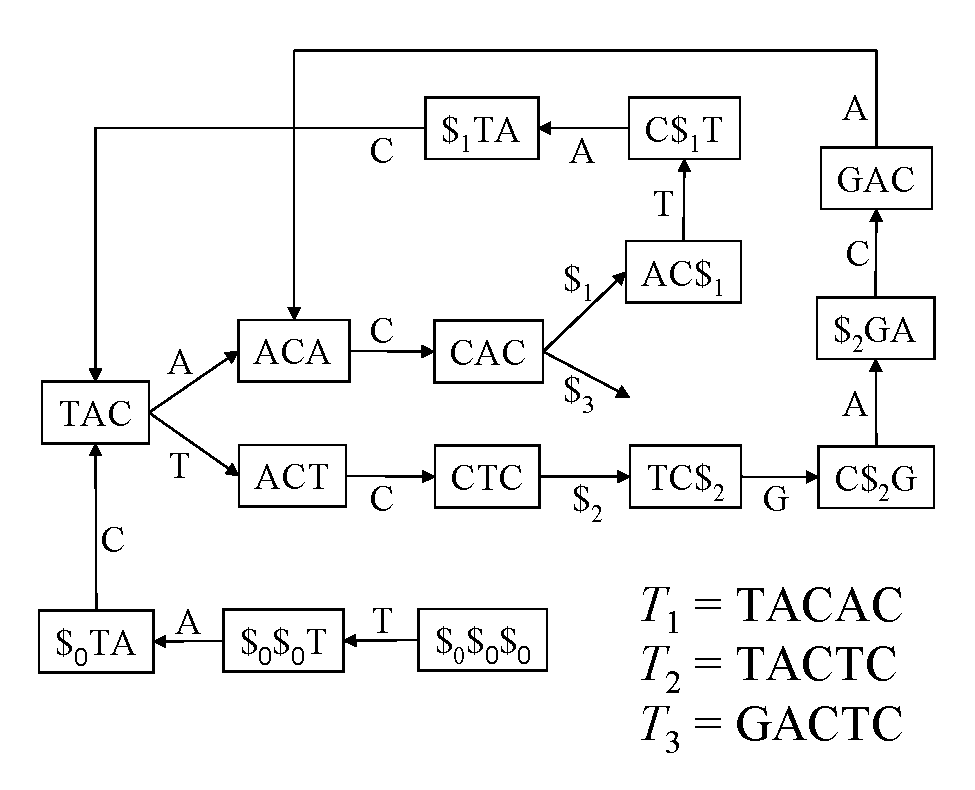
\includegraphics[scale=0.70]{fig3.eps} %PS
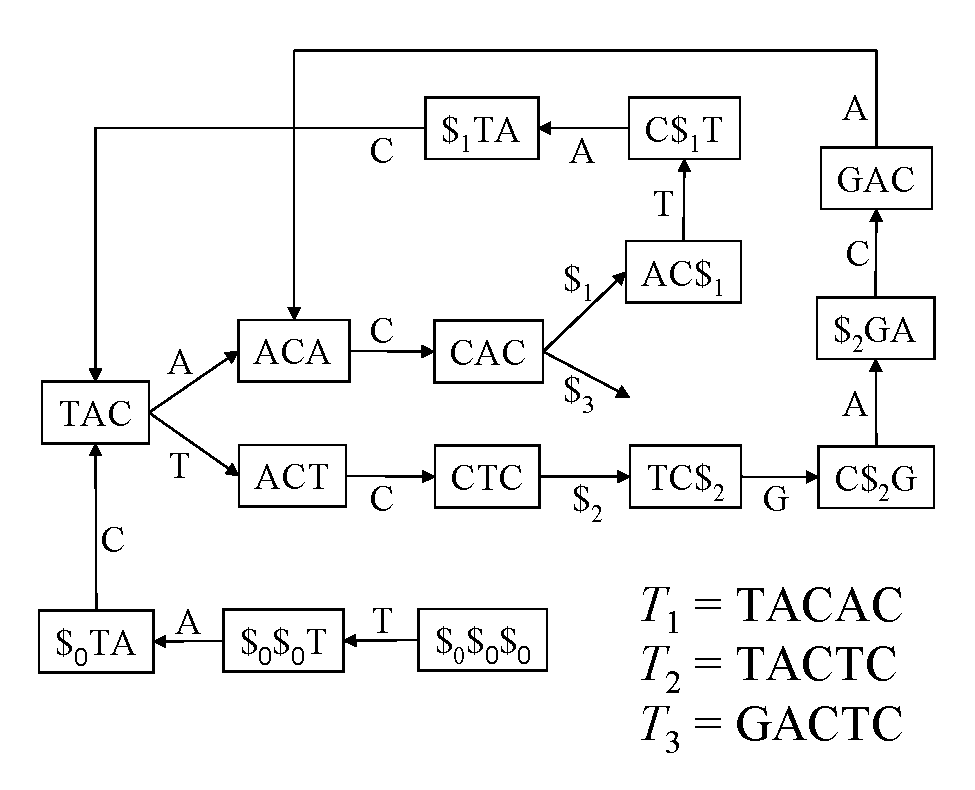
\includegraphics[scale=0.70]{fig3}
\caption{The $3$-dimensional de Bruijn graph of strings `TACAC', `TACTC', and
`GACTC'.}
\label{fig:debruijn}
\end{center}
\end{figure}

\cite{ICTFM12} introduced the {\em colored de Bruijn graph}, a variant of the classical structure, which is aimed at ``detecting and genotyping simple and complex genetic variants in an individual or population.'' The edge structure of the colored de Bruijn graph is the same as the classic structure, but now to each vertex ($(k - 1)$-mer) and edge ($k$-mer)
% FIXME: node coloring (CORTEX) looses information preserved in edge coloring(VARI), should we discuss this?  i.e. two nodes with the same color may or may not have a connecting edge with that color, but if you only color the nodes, you can't tell which is the case
is associated a list of colors corresponding to the samples in which the vertex or edge label exists. More specifically, given a set of $n$ samples, there exists a set $\mathcal{C}$ of $n$ colors $c_1, c_2, .., c_n$ where $c_i$ corresponds to sample $i$ and all $k$-mers and $(k-1)$-mers that are contained in sample $i$ are colored with $c_i$. A {\em bubble} in this graph corresponds to an undirected cycle, and is shown to be indicative of biological variation by \cite{ICTFM12}. 
{\sc Cortex}, the implementation of \cite{ICTFM12}, uses the colored de Bruijn graph to develop a method of assembling multiple genomes simultaneously, without losing track of the individuals from which $(k - 1)$-mers (and $k$-mers) originated. This graph is derived from either multiple reference genomes, multiple samples, or a combination of both.

Variant information of an individual or population can be deduced from structure present in the colored de Bruijn graph and the colors of each $k$-mer.
As implied by \cite{ICTFM12}, the ultimate intended use of colored de Bruijn graphs is to apply it to massive, population-level sequence data that is now abundant due to next generation sequencing technology (NGS) and multiplexing. These technologies have enabled production of sequence data for large populations, which has led to ambitious sequencing initiatives that aim to study genetic variation for agriculturally and bio-medically important species.  These initiatives include the {\em Genome 10K} project that aims to sequence the genomes of 10,000 vertebrate species~\citep{Haussler:2009}, the {\em iK5} project~\citep{Robinson:2011}, the 150 Tomato Genome ReSequencing project~\citep{tomato1,tomato2}, and the 1001 Arabidopsis project, a worldwide initiative to sequence cultivars of {\em Arabidopsis}~\citep{arabidopsis}.   Given the large number of individuals and sequence data involved in these projects, it is imperative that the colored de Bruijn graph can be stored and traversed in a space- and time-efficient manner.
 

\section{Rank and Select}
 \label{sec:rank} Two basic operations used in almost
every succinct and compressed data structure are {\em rank} and {\em select}.
Given a sequence (string) $S[1,n]$ over an alphabet $\Sigma =
\{1,\ldots,\sigma\}$, a character $c \in \Sigma $, and integers $i$,$j$,
$\rank_c(S,i)$ is the number of times that $c$ appears in $S[1,i]$, and
$\select_c(S,j)$ is the position of the $j$-th occurrence of $c$ in $S$.
%There is a great variety of techniques to answer these queries, with
%suitability depending on the nature of the sequence, for example, on whether or
%not it will be compressed and on the size of the alphabet.
For a binary string $B[1,n]$, the classic solution for rank and
select~\cite{Mun96} is built upon the input sequence, requiring $o(n)$
additional bits.  Generally, $\rank_1$ and $\select_1$ are considered the
default rank and select queries.  More advanced solutions
(e.g.~\cite{bitvector}) achieve zero-order compression of $B$,
%For example, the several structures (e.g.~\cite{bitvector}), (see
%also~\cite{kkp2014}), 
representing it in just $nH_0(B) + o(n)$ bits of space, and supporting $\rank$
and $\select$ operations in constant time. 
%Several practical implementations and improvements of RRR exists (see,
%e.g.,~\cite{kkp2014}).

\section{Wavelet Trees} \label{sec:WVT} To support rank and select on larger
alphabet strings, the wavelet tree~\cite{ggv2003,n2013} is a commonly used data
structure that occupies $n\log\sigma + o(n\log\sigma)$ bits of space and
supports $\rank$ and $\select$ queries in $\Oh{\log\sigma}$ time.  Wavelet trees
also support a variety of more complex queries on the underlying string (see,
e.g.~\cite{gnp2012}), in $\Oh{\log\sigma}$ time, and we will make use of some of
this functionality in Section~\ref{sec:implementing}.


%Our data structure for colored de Bruijn graphs is based on a succinct representation of individual de Bruijn graphs that was introduced by \cite{BOSS12} and which we refer to as the BOSS representation from the authors' initials.  The BOSS representation was in turn based on an adaptation of \cite{FM05} FM-indexes.  Before getting to our description of the succinct colored de Bruijn graph data structure, 
%In the rest of this section 
%we first describe FM-indexes and then explain the BOSS representation.
%Our explanation of BOSS is particularly simple and may be of independent interest to those wanting to better understand that data structure.
% This new take on BOSS was key to our development of our succinct colored de Bruijn graph. 
% Travis: No it wasn't, it came afterward. :o)

\section{FM-indexes}
\label{subsec:fm-indexes}

Consider a string $S$.  Let $F$ be the list of $S$'s characters sorted lexicographically by the suffixes starting at those characters, and let $L$ be the list of $S$'s characters sorted lexicographically by the suffixes starting immediately after those characters.  (The names $F$ and $L$ are standard for these lists.)  If \(S [i]\) is in position $p$ in $F$ then \(S [i - 1]\) is in position $p$ in $L$.  Moreover, if \(S [i] = S [j]\) then \(S [i]\) and \(S [j]\) have the same relative order in both lists; otherwise, their relative order in $F$ is the same as their lexicographic order.  This means that if \(S [i]\) is in position $p$ in $L$ then, assuming arrays are indexed from 0 and $\prec$ denotes lexicographic precedence, in $F$ it is in position
%\begin{multline*}
  \[|\{h\,:\,S [h] \prec S[i]\}| + |\{h\,:\,L [h] = S [i],\ h \leq p\}| - 1\,.\]
%  \end{multline*}
Finally, notice that the last character in $S$ always appears first in $L$.  It follows that we can recover $S$ from $L$, which is the famous Burrows-Wheeler Transform (BWT)~\citep{BW94} of $S$.

The BWT was introduced as an aid to data compression: it moves characters followed by similar contexts together and thus makes many strings encountered in practice locally homogeneous and easily compressible.  \cite{FM05} realized it could also be used for indexing because, if we know the range \(\BWT (S) [i..j]\) occupied by characters immediately preceding occurrences of a pattern $P$ in $S$, then we can compute the range \(\BWT (S) [i'..j']\) occupied by characters immediately preceding occurrences of \(c P\) in $S$, for any character $c$, since
\begin{eqnarray*}
i' & = & |\{h\,:\,S [h] \prec c\}| + |\{h\,:\,S [h] = c, h < i\}|\\
j' & = & |\{h\,:\,S [h] \prec c\}| + |\{h\,:\,S [h] = c, h \leq j\}| - 1\,.
\end{eqnarray*}
Notice \(j' - i' + 1\) is the number of occurrences of \(c P\) in $S$.  The essential components of an FM-index for $S$ are, first, an array storing \(|\{h\,:\,S [h] \prec c\}|\) for each character $c$ and, second, a rank data structure for \(\BWT (S)\) that quickly tells us how often any given character occurs up to any given position\footnote{Given a sequence (string) $S[1,n]$ over an alphabet $\Sigma = \{1,\ldots,\sigma\}$, a character $c \in \Sigma $, and an integer
$i$, $\rank_c(S,i)$ is the number of times that $c$ appears in $S[1,i]$.}.  
To be able to locate the occurrences of patterns in $S$ (in addition to just counting them), we can use a sampled suffix array of $S$ and a bitvector indicating the positions in \(\BWT (S)\) of the characters preceding the sampled suffixes.

